\documentclass{article}

\usepackage[pdftex]{graphicx}
\usepackage[czech]{babel}
\usepackage[utf8]{inputenc}
\usepackage{enumitem}
\usepackage{amsmath}
\usepackage{url}
\usepackage{listings}
\usepackage{caption}
\usepackage{gensymb}
\usepackage[usenames,dvipsnames,svgnames,table]{xcolor}

\usepackage[pdftex]{hyperref}
\hypersetup{colorlinks=true,
  unicode=true,
  linkcolor=black,
  citecolor=black,
  urlcolor=black,
  bookmarksopen=true}

\usepackage{xcolor}
\colorlet{mygray}{black!30}
\colorlet{mygreen}{green!60!blue}
\colorlet{mymauve}{red!60!blue}
\lstset{
	backgroundcolor=\color{gray!10},  
	basicstyle=\ttfamily,
	columns=fullflexible,
	breakatwhitespace=false,      
	breaklines=true,                
	captionpos=b,                    
	commentstyle=\color{mygreen}, 
	extendedchars=true,              
	frame=single,                   
	keepspaces=true,             
	keywordstyle=\color{blue},      
	language=c++,                 
	numbers=none,                
	numbersep=5pt,                   
	numberstyle=\tiny\color{blue}, 
	rulecolor=\color{mygray},        
	showspaces=false,               
	showtabs=false,                 
	stepnumber=5,                  
	stringstyle=\color{mymauve},    
	tabsize=3,                      
	title=\lstname                
}

\usepackage[numbers,sort&compress]{natbib}

\newcommand*\justify{
  \fontdimen2\font=0.4em
  \fontdimen3\font=0.2em
  \fontdimen4\font=0.1em
  \fontdimen7\font=0.1em
  \hyphenchar\font=`\-
}

\makeatletter
\def\subtitle#1{\gdef\@subtitle{#1}}
\def\maketitle{\begin{titlepage}%
		\let\footnotesize\small
		\let\footnoterule\relax
		\let \footnote \thanks
		\null\vfil
		\vskip 60\p@
		\begin{center}%
			{\LARGE \@title \par}%
			\vskip 1.5em% Added this
			{\Large \@subtitle \par}% and this
			\vskip 3em%
			{\large
				\lineskip .75em%
				\begin{tabular}[t]{c}%
					\@author
				\end{tabular}\par}%
			\vskip 1.5em%
			{\large \@date \par}%       % Set date in \large size.
		\end{center}\par
		\@thanks
		\vfil\null
	\end{titlepage}%
	\setcounter{footnote}{0}%
	\global\let\thanks\relax
	\global\let\maketitle\relax
	\global\let\@thanks\@empty
	\global\let\@author\@empty
	\global\let\@date\@empty
	\global\let\@title\@empty
	\global\let\title\relax
	\global\let\author\relax
	\global\let\date\relax
	\global\let\and\relax
}
\makeatother

\title{KIV-DPP-01}
\subtitle{Dokumentace rozšiřující desky}
\author{Martin Úbl}
\date{1. září 2021}

\begin{document}

\maketitle



\section{Přehled}

\begin{figure}[ht]
	\centering
	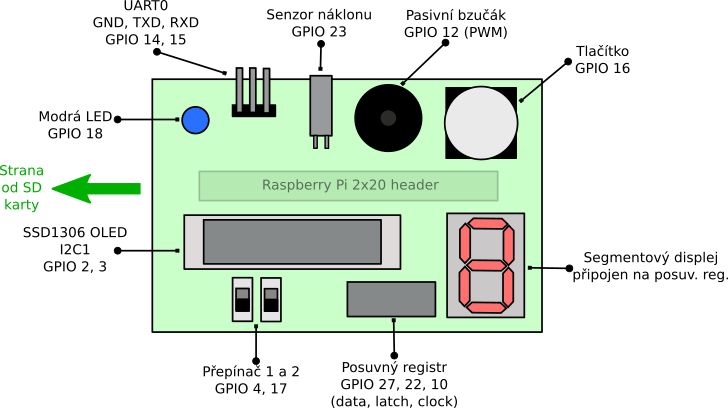
\includegraphics[width=1.0\linewidth]{kiv-dpp-01.png}
\end{figure}

Deska KIV-DPP-01 (KIV Deska Plná Periferií rev. 01) obsahuje následující sadu periferií:
\begin{itemize}
	\item Modrá LED (GPIO 18)
	\item UART header (GPIO 14, 15)
	\item Senzor náklonu (GPIO 23)
	\item Pasivní bzučák (GPIO 12)
	\item Tlačítko (GPIO 16)
	\item Sedmi-segmentový displej (přímo připojen na posuvný registr)
	\item Posuvný registr 74HC595N (GPIO 27, 22, 10)
	\item Polohový přepínač 1 (GPIO 4)
	\item Polohový přepínač 2 (GPIO 17)
	\item SSD1306 OLED displej (I2C1; GPIO 2, 3)
\end{itemize}

\newpage

\section{Zapojení}

Deska obsahuje 2x20-pin header, který přímo pasuje do pinového protikusu na straně Raspberry Pi. Důležité je dodržet orientaci rozšiřující desky vůči Raspberry Pi -- LED na rozšiřující desce se musí nacházet na straně, kde se na hostitelské desce nachází slot na SD kartu. Posuvný registr a segmentový displej se pak nachází na straně, kde má hostitelská deska umístěné USB konektory.

\section{LED}

\begin{itemize}
	\item Barva: modrá (455-465 nm)
	\item GPIO: 18
	\item Zapojení: IN - LED - GND
	\item Spotřeba: max. 20 mA
	\item Svítivost: max. 3000 mcd
\end{itemize}

Klasická modrá LED, anoda je vyvedená na GPIO pin 18, katoda na GND.

\section{UART header}

\begin{itemize}
	\item GPIO: 14 (TXD), 15 (RXD)
	\item Zapojení: přímé
\end{itemize}

Header pro připojení UART terminálu, např. USB-TTL převodník do hostitelského PC. Piny jsou zleva (od LED) zapojeny na: GND, TXD, RDX. Zapojení je přímé -- do hostitelského počítače tedy musí být překřížené.

\section{Senzor náklonu}

\begin{itemize}
	\item GPIO: 23
	\item Zapojení: pull-up
	\item Datasheet: \url{http://home.zcu.cz/~ublm/files/os/SW-520D.pdf}
\end{itemize}

Kuličkový senzor náklonu SW-520D, který je připájený úmyslně pod úhlem cca 15\degree, dovede detekovat, zda je zařízení v horizontální nebo vertikální poloze (resp. \uv{půl-poloze} vzhledem k povaze senzoru).

\section{Pasivní bzučák}

\begin{itemize}
	\item GPIO: 12
	\item Zapojení: přímé
	\item Odpor: 16 $\Omega$
\end{itemize}

Pasivní bzučák zapojený na GPIO 12. Bzučák je pasivní, takže nemá interní oscilátor -- je nutné ho tedy řídit PWM signálem.

\section{Tlačítko}

\begin{itemize}
	\item GPIO: 16
	\item Zapojení: pull-up
\end{itemize}

Klasické tlačítko s plastovou čepičkou.

\section{Sedmi-segmentový displej}

\begin{itemize}
	\item GPIO: -
	\item Zapojení: společná katoda, IN - LED - 3.3V
	\item Spotřeba: max. 15 mA
	\item Datasheet: \url{http://home.zcu.cz/~ublm/files/os/5161AS.pdf}
\end{itemize}

Sedmi-segmentový displej 5161AS je připojený na výstupy posuvného registru. Nelze jej tedy ovládat samostatně. Zapojení je se společnou katodou.

Zobrazovací jednotka je na výstupy posuvného registru připojena následovně:
\begin{figure}[ht!]
	\centering
	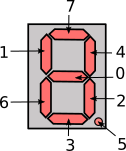
\includegraphics[width=0.3\linewidth]{kiv-dpp-01-segments.png}
\end{figure}

\section{Posuvný registr}

\begin{itemize}
	\item GPIO: 27 (data), 22 (latch), 10 (clock)
	\item Zapojení: přímé
	\item Datasheet: \url{http://home.zcu.cz/~ublm/files/os/74HC565.pdf}
\end{itemize}

Posuvný registr 74HC595N je vstupy zapojen přímo na GPIO 27 (datový pin), 22 (latch pin, přepnutí banku) a 10 (časovací signál). Výstupy jsou zapojeny na vstupy sedmi-segmentového displeje.

\section{Polohové přepínače}

\begin{itemize}
	\item GPIO: 4 (př. 1), 17 (př. 2)
	\item Zapojení: pull-down
\end{itemize}

Běžné malé nezávisle zapojené polohové přepínače.

\section{OLED displej}

\begin{itemize}
	\item I2C: kanál 1
	\item GPIO: 2 (SDA), 3 (SCL)
	\item Zapojení: přímé
	\item Typ: monochromatický (modrá nebo bílá)
	\item Velikost matice: 128x32 bodů
	\item Datasheet: \item Datasheet: \url{http://home.zcu.cz/~ublm/files/os/SSD1306.pdf}
\end{itemize}

Displej SSD1306 je přímo připojený na piny 2 a 3, na kterých na hostitelské desce operuje I2C kanál 1. Protokol pro ovládání displeje je shodný pro všechny displeje z řady SSD1306 (všechny rozměry). Body displeje mohou svítit buď bílou nebo modrou barvou.

\end{document}























